% Document settings
\documentclass[a4paper,11pt]{article}

% Packages
  % math formulas
\usepackage{amsmath,amsthm,amssymb}
  % graphics
\usepackage{graphicx}
\usepackage{wrapfig}
  % plots
\usepackage{pgfplots}
  % other
\usepackage[warn]{mathtext}
\usepackage{cmap}
\usepackage[T1,T2A]{fontenc}
\usepackage[utf8]{inputenc}
\usepackage[english,russian]{babel}

% Package settings
%% graphicx
\graphicspath{{Pictures/}}
\DeclareGraphicsExtensions{.pdf,.png,.jpg}
%% pgfplots
\pgfplotsset{width=10cm,compat=1.9}

% Title
\title{Отчет о выполнении работы №1.4.1\newlineИзучение экспериментальных погрещностей на примере физического маятника}
\author{Воейко Андрей Александрович, Б01-109}
\date{Долгопрудный, 2021}

% Document
\begin{document}
\maketitle
\newpage
\section{Аннотация}
В работе проверяется справедливость формулы для периода колебаний физического маятника, теоремы Гюйгенса, определяется ускорение свободного падения.
\section{Теоретические сведения}
На рисунке~\ref{fig:img1} изображен стрежень без груза. Момент инерции относительно точки подвеса вычисляется по формуле~\ref{eq1}.
\begin{wrapfigure}{r}{0.2\textwidth}
  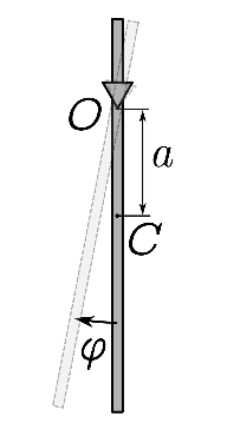
\includegraphics[scale = 0.5]{pic1.png}
  \caption{Стержень в качнестве физического маятника.}
  \label{fig:img1}
\end{wrapfigure}
\begin{equation}    \label{eq1}
  I_{0} = \frac{m_{0}l^{2}}{12} + m_{0}a^{2},
\end{equation}
где $I$ -- момент инерции, $l$ -- длина стержня, $m_{0}$ -- масса стержня с призмой, $a$ -- расстояние от точки подвеса до центра масс.\newline
Возвращающрий момент силы тяжести равен:
\begin{equation}    \label{eq2}
  M = -m_{0}g a \sin{\phi} \approx -m_{0}g a \phi.
\end{equation}
Таким образом,
$$\frac{d^{2}\phi}{dt^{2}} \sim - \phi.$$
Период цолебаний можно найти по формуле~\ref{eq3}.
\begin{equation}    \label{eq3}
  T = 2 \pi \sqrt{\frac{I}{m_{0}ga}\ } = 2 \pi \sqrt{\frac{\frac{l^{2}}{12} + a^{2}}{ga}\ }
\end{equation}
Приведенная длина физического маятника $l_{пр}$ (взята из $T = 2 \pi \sqrt{\frac{l}{g}\ }$):
\begin{equation}    \label{eq4}
  l_{пр} = a + \frac{l^{2}}{12a}.
\end{equation}
Рсстояние дто груза до центра масс $x_{ц}$:
\begin{equation}    \label{eq5}
  x_{ц} = \frac{m_{0}x_{ц 0} + m_{г}y}{m_{0} + m_{г}},
\end{equation}
где $m_{0}$ -- масса стержня с призмой, $x_{ц,0}$ -- расстояние от центра масс без груза до призмы, $m_{г}$ -- масса груза, $y$ -- расстояние от призмы до ц. м. груза.\newline
Поскольку груз имеет сложную форму, следует один раз вычислить $x_{ц}$ для первого измерения, а потом находить ее изменение по изменению $y$ из формулы~\ref{eq5}. Тогд апериод колебаний составит:
\begin{equation}    \label{eq6}
  T = 2 \pi \sqrt{\frac{I_{0} + m_{г} y^{2}}{(m_{0} + m_{г}) g x_{ц}}}.
\end{equation}
Отсюда вывводим $g$:
\begin{equation}    \label{eq7}
  g = \frac{I_{0} + m_{г}y^{2}}{(m_{0} + m_{г}) x_{ц}} \frac{4 \pi^{2}}{T^{2}} = \frac{4 \pi^{2}}{T^{2}} \frac{m_{0}(\frac{l^{2}}{12} + a^{2}) + m_{г} y^{2}}{m_{0}x_{ц,0} + m_{г}y}.
\end{equation}
\section{Оборудование и экспериментальная установка}
\section{Результаты измерений и обработка данных}
\subsection{Результаты измерений}
\subsection{Обработка данных}
\section{Выводы}
\end{document}
